\documentclass[a4paper,12pt]{article}
\usepackage[utf8x]{inputenc} % Codifica UTF-8
\usepackage[italian]{babel} % Lingua italiana
\usepackage[T1]{fontenc}
\usepackage{amsmath} % Simboli matematici
\usepackage{siunitx} % Unità di misura
\usepackage{listings} % Inserimento codice
\usepackage{graphicx} % Inserimento immagini
\usepackage{caption} % Didattiche delle figure
\usepackage{hyperref} % Riferimenti ipertestuali
\usepackage{xcolor} % Definizione dei colori
\usepackage{mdframed} % Per le scatole colorate

% Configurazione per il codice Python
\lstset{ 
  language=Python,
  backgroundcolor=\color{white}, 
  basicstyle=\ttfamily\footnotesize, % font size and typewriter
  breaklines=true, % automatic line breaking
  frame=single, % adds a frame around the code
  numbers=left, % adds line numbers on the left
  numberstyle=\tiny\color{gray}, % style for line numbers
  keywordstyle=\color{blue}, % color for keywords
  commentstyle=\color{green}, % color for comments
  stringstyle=\color{red}, % color for strings
  captionpos=b, % position of the caption (b=bottom)
}


\title{Analisi Statistica dei Dati Sperimentali}
\author{Laboratorio di Fisica}
\date{}

\begin{document}

\maketitle
\tableofcontents
\section{Introduzione}
In questo capitolo esploreremo l'analisi statistica dei dati sperimentali utilizzando Python. Gli argomenti trattati includeranno la gestione delle misure come variabili casuali, la funzione di distribuzione normale, l'uso di matplotlib per la visualizzazione dei dati e la regressione lineare. Eseguiremo anche un esempio completo per il calcolo dell'accelerazione di gravit\'a.

\section{Misure come Variabili Casuali}
Le misure sperimentali sono trattate come variabili casuali, il che implica che i valori misurati sono soggetti a variazioni casuali dovute a errori di misurazione e condizioni sperimentali.

\section{Distribuzione Normale e Stima dei Parametri}

La distribuzione normale è spesso utilizzata per modellare errori e incertezze nelle misure. La funzione di distribuzione normale è definita da due parametri principali: la media e la deviazione standard.

\subsection{Esempio di Stima dei Parametri}

Consideriamo i seguenti dati sperimentali:

\[
\begin{array}{c|c}
\text{Misura} & \text{Valore} \\
\hline
1 & 4.900 \\
2 & 19.600 \\
3 & 44.100 \\
4 & 78.400 \\
5 & 122.500 \\
\end{array}
\]

Il codice Python per calcolare la media e la deviazione standard è:

\begin{lstlisting}[caption={Calcolo della media e deviazione standard}]
import numpy as np

# Dati sperimentali
dati = np.array([4.900, 19.600, 44.100, 78.400, 122.500])

# Calcolo della media e della deviazione standard
media = np.mean(dati)
deviazione_standard = np.std(dati, ddof=1)

print(f"Media: {media:.3f} m")
print(f"Deviazione standard: {deviazione_standard:.3f} m")
\end{lstlisting}

\section{Uso di Matplotlib per la Visualizzazione dei Dati}

Matplotlib è una libreria potente per la creazione di grafici in Python. Di seguito è riportato un esempio di come realizzare un grafico delle misure sperimentali con barre di errore.

\subsection{Esempio di Grafico}

Consideriamo l'esempio dell'accelerazione di gravità con i seguenti dati:

\[
\begin{array}{c|c}
\text{Tempo (s)} & \text{Distanza (m)} \\
\hline
1.0 & 4.900 \\
2.0 & 19.600 \\
3.0 & 44.100 \\
4.0 & 78.400 \\
5.0 & 122.500 \\
\end{array}
\]

Per mostrare le barre di errore, inseriamo nel codice errori volutamente molto grandi. Si noti inoltre che abbiamo modificato la grandezza dei punti col parametro \textbf{markersize}, la larghezza dei segmenti per le barre con il parametro \textbf{capsize}, e la dimensione del grafico con l'istruzione \textbf{plt.figure(figsize=(12, 9))}.

\begin{lstlisting}[caption={Grafico delle misure sperimentali con barre di errore}]
import numpy as np
import numpy as np
import matplotlib.pyplot as plt

# Dati sperimentali
tempo = np.array([1.0, 2.0, 3.0, 4.0, 5.0])
distanza = np.array([4.900, 19.600, 44.100, 78.400, 122.500])
error_distanza = np.array([1, 2, 3, 1, 4])  # Errori aumentati
error_t2 = np.array([1, 1, 1, 1, 1])

# Configurazione per usare LaTeX in Matplotlib


# Creazione del grafico con dimensioni maggiori e punti più piccoli
plt.figure(figsize=(12, 9))  # Dimensioni della figura
plt.errorbar(tempo**2, distanza, yerr=error_distanza, xerr=error_t2, fmt='o', label='Dati sperimentali', capsize=5, elinewidth=2, markersize=6)
plt.title(r'Misurazione dell\'Accelerazione di gravità', fontsize=16)
plt.xlabel(r'Tempo al quadrato $(s^2)$', fontsize=14)
plt.ylabel(r'Distanza (m)', fontsize=14)
plt.legend()
plt.grid(True)
plt.savefig('grafico_misure.png')  # Salvataggio dell'immagine
plt.show()



\end{lstlisting}

Nella figura \ref{fig:grafico_misure} è mostrato il grafico risultante.

\begin{figure}[h!]
    \centering
    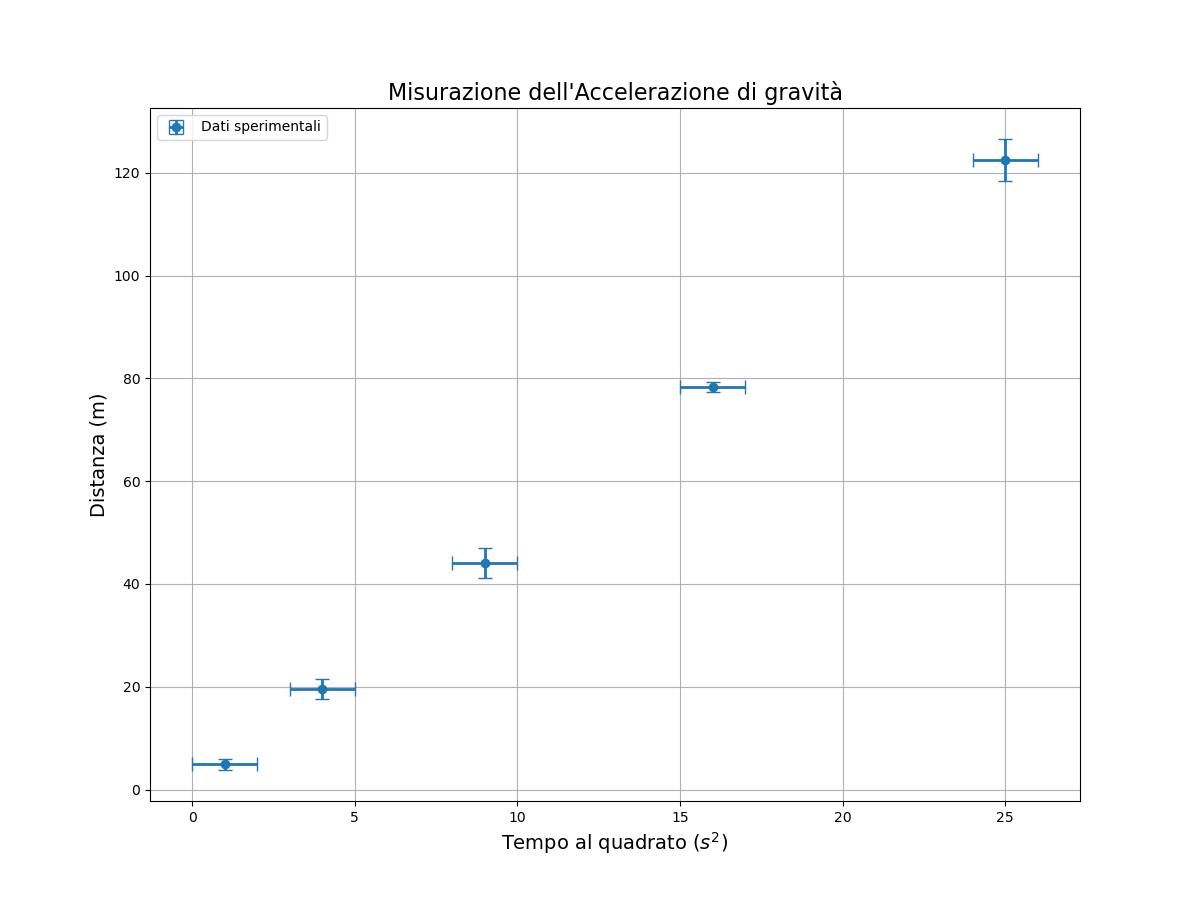
\includegraphics[width=\textwidth]{grafico_misure.png}
    \caption{Grafico delle misure sperimentali con barre di errore.}
    \label{fig:grafico_misure}
\end{figure}


\section{Regressione Lineare}
In fisica, il moto uniforme è un tipo di moto in cui un oggetto si sposta con velocità costante. Questo significa che la distanza percorsa dall'oggetto è proporzionale al tempo impiegato. La relazione tra spazio \( y \) e tempo \( x \) in un moto uniforme può essere espressa tramite la seguente equazione lineare:

\[
y = v \cdot x + s_0
\]

dove:
\begin{itemize}
    \item \( v \) è la velocità costante dell'oggetto (pendenza della retta).
    \item \( s_0 \) è la posizione iniziale dell'oggetto (intercetta della retta).
\end{itemize}

L'obiettivo è trovare i parametri \( v \) e \( s_0 \) che meglio rappresentano i dati sperimentali. Utilizzando una regressione lineare, possiamo ottenere questi parametri adattando una retta ai dati.

\subsection{Tabella dei Dati}

Per l'analisi, consideriamo i seguenti dati sperimentali raccolti per tempo e spazio:

\begin{table}[h!]
    \centering
    \begin{tabular}{|c|c|}
    \hline
    \textbf{Tempo (\si{\second})} & \textbf{Spazio (\si{\meter})} \\
    \hline
    1.0 & 2.0 \\
    2.0 & 4.0 \\
    3.0 & 6.0 \\
    4.0 & 8.0 \\
    5.0 & 10.0 \\
    \hline
    \end{tabular}
    \caption{Dati sperimentali di tempo e spazio.}
    \label{tab:dati}
\end{table}

\subsection{Regressione Lineare}

La regressione lineare cerca di adattare una retta ai dati sperimentali, trovando i parametri \( a \) e \( b \) che minimizzano la somma dei quadrati delle differenze tra i valori osservati e quelli previsti dalla retta. In questo caso, la retta di regressione è data da:

\[
y = a \cdot x + b
\]

dove:
\begin{itemize}
    \item \( a \) è la pendenza della retta, che rappresenta la velocità \( v \).
    \item \( b \) è l'intercetta, che rappresenta la posizione iniziale \( s_0 \).
\end{itemize}

\subsection{Uso di Python per la Regressione Lineare}
Per calcolare i parametri della retta di regressione e il loro errore, utilizziamo il modulo \texttt{scipy.optimize.curve\_fit} di Python, che permette di adattare una funzione ai dati sperimentali. La funzione \texttt{curve\_fit} ritorna i parametri ottimizzati e le loro deviazioni standard. Utilizziamo anche \texttt{matplotlib} per visualizzare i dati e la retta di regressione.


Ecco il codice Python utilizzato:

\begin{lstlisting}
import numpy as np
from scipy.optimize import curve_fit
import matplotlib.pyplot as plt
# Dati sperimentali
tempo = np.array([1.0, 2.0, 3.0, 4.0, 5.0])
spazio = np.array([2.0, 4.0, 6.0, 8.0, 10.0])

# Definizione della funzione di modello lineare
def linear_model(x, a, b):
    return a * x + b

# Fitting dei dati
params, params_covariance = curve_fit(linear_model, tempo, spazio)

# Estrazione dei parametri
pendenza, intercetta = params
pendenza_error, intercetta_error = np.sqrt(np.diag(params_covariance))

print(f"Pendenza: {pendenza:.3f} ± {pendenza_error:.3f}")
print(f"Intercetta: {intercetta:.3f} ± {intercetta_error:.3f}")

# Creazione del grafico
plt.figure(figsize=(8, 6))
plt.scatter(tempo, spazio, label='Dati sperimentali')
plt.plot(tempo, linear_model(tempo, *params), 'r-', label='Retta di regressione')
plt.xlabel('Tempo (\si{\second})')
plt.ylabel('Spazio (\si{\meter})')
plt.title('Fitting Lineare')
plt.legend()
plt.grid(True)
plt.savefig('regressione_lineare.png')  # Salvataggio dell'immagine
plt.show()
\end{lstlisting}

\subsection{Output del Codice Python}

L'output del codice Python è il seguente:

\begin{mdframed}[backgroundcolor=lightgray, linecolor=black, linewidth=1pt]
\textbf{Pendenza}: \(2.020 \pm 0.083 \, \si{\meter\per\second}\) \\
\textbf{Intercetta}: \(0.200 \pm 0.276 \, \si{\meter}\)
\end{mdframed}

\textbf{Pendenza}: La pendenza della retta di regressione è \(2.020 \pm 0.083 \, \si{\meter\per\second}\). Questo valore rappresenta la velocità media del moto. L'errore associato indica l'incertezza nella determinazione della pendenza, che riflette la variabilità dei dati sperimentali rispetto alla retta di regressione.

\textbf{Intercetta}: L'intercetta della retta di regressione è \(0.200 \pm 0.276 \, \si{\meter}\). Questo valore rappresenta la posizione iniziale, cioè il valore di \(y\) quando \(x\) è zero. L'errore associato all'intercetta indica l'incertezza nella misura del punto in cui la retta di regressione interseca l'asse delle ordinate. Questo valore può dare indicazioni sul punto di partenza del movimento descritto dai dati.



Di seguito , in figura \ref{fig:regressione_lineare} è mostrato il grafico della regressione lineare che visualizza i dati sperimentali insieme alla retta di regressione ottenuta.

\begin{figure}[h!]
    \centering
    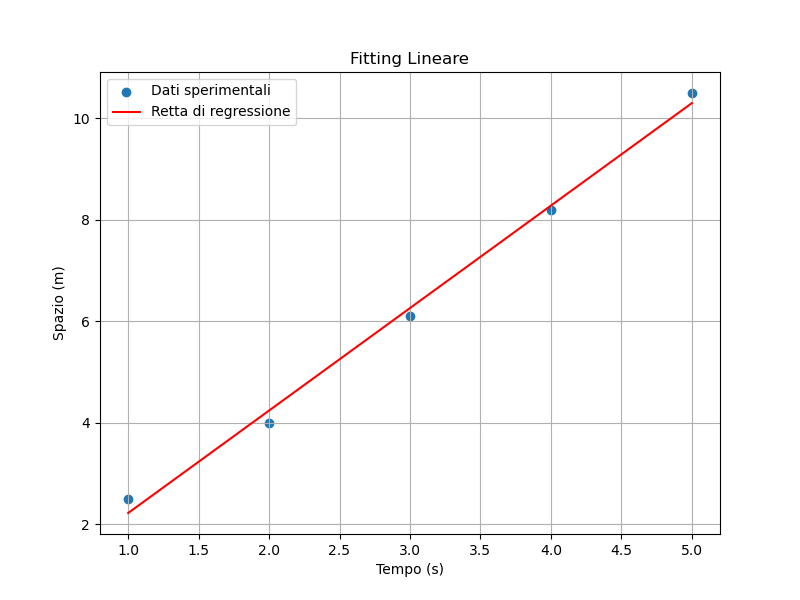
\includegraphics[width=0.8\textwidth]{regressione_lineare.png}
    \caption{Grafico della regressione lineare: i dati sperimentali sono mostrati come punti, e la retta di regressione è mostrata in rosso.}
    \label{fig:regressione_lineare}
\end{figure}

\end{document}
